\chapter{Shaft Design}

\section{Choose material}
For moderate load, carbon steel AISI 1035 \cite{aisi1035} is selected to design the shafts:
\[\text{HB}183, \sigma_b = 585\unit{MPa}, \sigma_{ch} = 370\unit{MPa} \]

\section{Loads on shafts}
In this chapter, a subscript convention shall be used for clarity. The rule of the convention is as follows:
\begin{itemize}
	\item a variable describing the mechanical drive's property on the shaft uses 2 numeric subscripts. The first subscript is the ordinal number of shafts. The second subscript is the ordinal number of mechanical drives (e.g. motor, gear, chain, belt).
	\item if a variable is of the shaft's property, it uses 1 numeric subscript.
	\item the location of a force on the shaft is specified with 1 capitalized letter after the numeric subscripts. On each shaft of this design problem, the letters $ A,B,C,D $ represent 4 critical sections from left to right.
	\item for a force vector, $ x,y,z $ are its algebraic values on $ x,y,z $-axis, respectively.
	\item at critical sections with a moment jump, 2 superscipts are used. The left side is $ ^- $ while the right side is $ ^+ $.
\end{itemize}
Therefore,
\begin{itemize}
	\item On shaft 1: the motor is labeled 1, the pinion is labeled 2.
	\item On shaft 2: the driving gear is labeled 1, the pinion is labeled 2.
	\item On shaft 3: the driving gear is labeled 1, the chain is labeled 2.
\end{itemize}
Applying this rule in force computation yields:\\

\begin{figure}[ht]
	\centering
	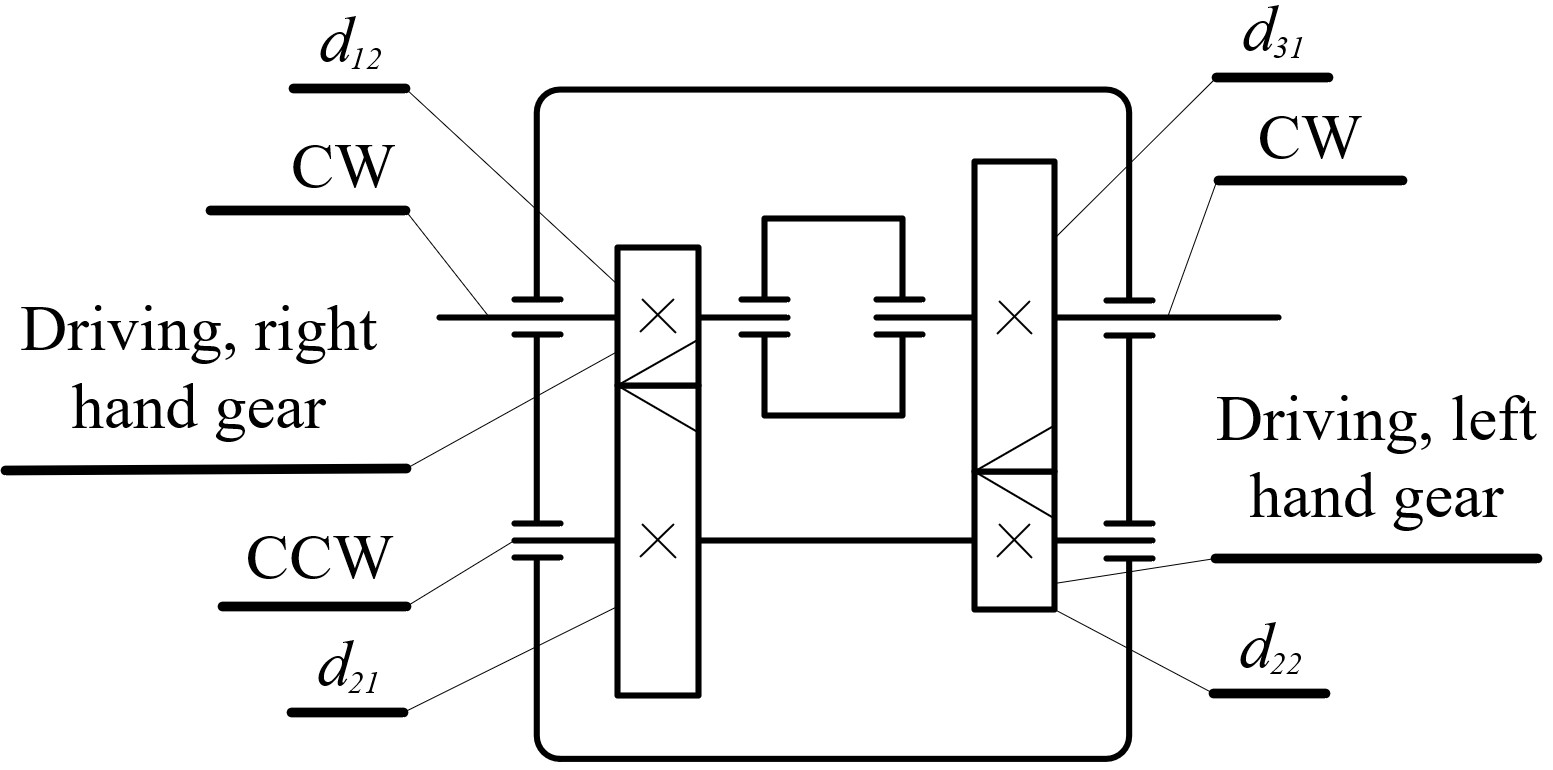
\includegraphics{states}
	\caption{Detailed description of the speed reducer}
	\label{states}
\end{figure}

Force from pinion 1:
\[
\begin{array}{ll}
F_{12x}& = c_{b12}c_{q12}\dfrac{2T_{sh1}}{d_{12}} = (+1)\times(-1)\times\dfrac{2\times 46423.73}{83.57} = -1111.06 \unitp{N}\\
F_{12y}& = -\dfrac{2T_{sh1}}{d_{12}}\dfrac{\tan\alpha_n}{\cos\beta_{12}} = -\dfrac{2\times 46423.73}{83.57}\times\dfrac{\tan 20^\circ}{\cos 11.11^\circ} = -412.12\unitp{N}\\
F_{12z}& = c_{b12}c_{q12}h_{r12}\dfrac{2T_{sh1}}{d_{12}}\tan \beta_{12} \\
&= (+1)\times(-1)\times(+1)\times\dfrac{ 2\times 46423.73}{83.57} \times\tan 11.11^\circ\\
& = -218.24 \unitp{N}
\end{array}
\]

Force from driven gear 1:
\[
\begin{array}{l}
F_{21x} = -F_{12x} = 1111.06 \unitp{N}\\
F_{21y} = -F_{12y} = 412.12 \unitp{N}\\
F_{21z} = -F_{12z} = 218.24 \unitp{N}\\
\end{array}
\]

Force from pinion 2:
\[
\begin{array}{ll}
F_{22x}& = c_{b22}c_{q22}\dfrac{2T_{sh2}}{d_{22}} = (+1)\times(+1)\times\dfrac{2\times 126093.30}{83.08} = 1117.61 \unitp{N}\\
F_{22y}& = -\dfrac{2T_{sh2}}{d_{22}}\dfrac{\tan\alpha_n}{\cos\beta_{22}} = -\dfrac{2\times 126093.30}{83.08}\times\dfrac{\tan 20^\circ}{\cos 12.84^\circ} = -1133.19\unitp{N}\\
F_{22z}& = c_{b22}c_{q22}h_{r22}\dfrac{2T_{sh2}}{d_{22}}\tan \beta_{22} \\
&= (+1)\times(+1)\times(-1)\times\dfrac{ 2\times 126093.30}{83.08} \times\tan 12.84^\circ\\
& = -691.82 \unitp{N}
\end{array}
\]

Force from driven gear 2:
\[
\begin{array}{l}
F_{31x} = -F_{22x} = -1117.61 \unitp{N}\\
F_{31y} = -F_{22y} = 1133.19 \unitp{N}\\
F_{31z} = -F_{22z} = 691.82 \unitp{N}\\
\end{array}
\]

where
\begin{itemize}
	\item $ F $ is the force exerting on the shaft,$ \unit{N} $.
	\item $ c_q $ is the rotation direction of the shaft from the shaft end. For counterclockwise rotations (CCW), $ c_q=+1 $; for clockwise rotations (CW), $ c_q=-1 $. In this case, shaft 1 is assumed to rotate clockwise.
	\item $ c_b $ is the state of the gear. For driving gears, $ c_b=+1 $; for driven gears, $ c_b=-1 $.
	\item $ h_r $ is the tooth direction. For right hand gears, $ h_r= +1$; for left hand gears, $ h_r=-1 $.
	\item $ \beta $ is the helix angle given in \textbf{Table \ref{chap4spec}} and \textbf{\ref{chap5spec}},$ ^\circ $.
	\item $ d $ is the diameter of the gear,$ \unit{mm} $. From \textbf{Table \ref{chap4spec}} and \textbf{\ref{chap5spec}},
	\[
	\begin{array}{l}
	d_{12}=83.57\unit{mm},d_{21}=236.43\unit{mm}\\
	d_{22}=83.08\unit{mm},d_{31}=236.92\unit{mm}
	\end{array}
	\]
	\item $ T_{sh1},T_{sh2} $ are given in \textbf{Table \ref{tab:my-table}}.
\end{itemize}

Let $  $

Let $ \alpha $ be the angle of the chain drive with respect to ground. From \textbf{Table \ref{chain}}'s description, the chain is parallel to ground, which makes $ \alpha = 0^\circ $.
\[
\begin{array}{l}
F_{32x} = F_{r32}\cos(\alpha) = 3741\cos(0) = 3741 \unitp{N}\\
F_{32y} = F_{r32}\sin(\alpha) = 3741\sin(0) = 0 \unitp{N}\\
\end{array}
\]

\section{Determination of shaft diameters at critical sections}
\subsection{Preliminary estimation of shafts diameter}
For input shaft, it is recommended to choose permissible torsion stress a small value $ [\tau] $ for the input shaft and a large value for the output shaft. From Equation 10.9 \cite{tk1}, the minimum nominal diameter of 3 shafts are
\[
\begin{array}{l}
d_1 \geq \sqrt[3]{\dfrac{5T_{sh1}}{[\tau_1]}} = \sqrt[3]{\dfrac{5\times 46423.73}{15}} = 24.92 \unitp{mm}\\
d_2 \geq \sqrt[3]{\dfrac{5T_{sh2}}{[\tau_2]}} = \sqrt[3]{\dfrac{5\times 126093.30}{20}} = 31.59 \unitp{mm}\\
d_3 \geq \sqrt[3]{\dfrac{5T_{sh3}}{[\tau_3]}} = \sqrt[3]{\dfrac{5\times 342486.86}{25}} = 40.92 \unitp{mm}
\end{array}
\]
where
\begin{itemize}
	\item $ d_1,d_2,d_3 $ are the diameters of shaft 1, 2, 3 respectively,$ \unit{mm} $.
	\item $ T_{sh1},T_{sh2},T_{sh3}$ are given in \textbf{Table \ref{tab:my-table}}.
\end{itemize}

Machining the gears integrally with the shaft is better suitable for precision special machines and production in large quantities. In this design, the scale is smaller and non-specialized. The gears are mounted on separate shafts, with the torque transmitted from the shaft to the gear through a key. The benefit of this setup is positive means of transmitting the torque while allowing easy assembly and disassembly \cite{mott_vavrek_wang_2018}.

Since the input shaft is connected with the motor shaft by a flexible coupling, the difference between 2 diameters must be within $ 20\% $ of the motor diameter $ d_{mo} $. Inspecting Table P1.7 for motor 4A132S4Y3, $ d_{mo}=42.00\unit{mm} $. Combining with Table 10.2 \cite{tk1} to obtain the nominal diameter of 3 shafts and the corresponding bearings width:
\[
\begin{array}{l}
d_1=35\unit{mm},d_2=35\unit{mm},d_3=45\unit{mm}\\
b_{O1}=21\unit{mm},b_{O2}=21\unit{mm},b_{O3}=25\unit{mm}
\end{array}
\]

\begin{figure}[ht]
	\centering
	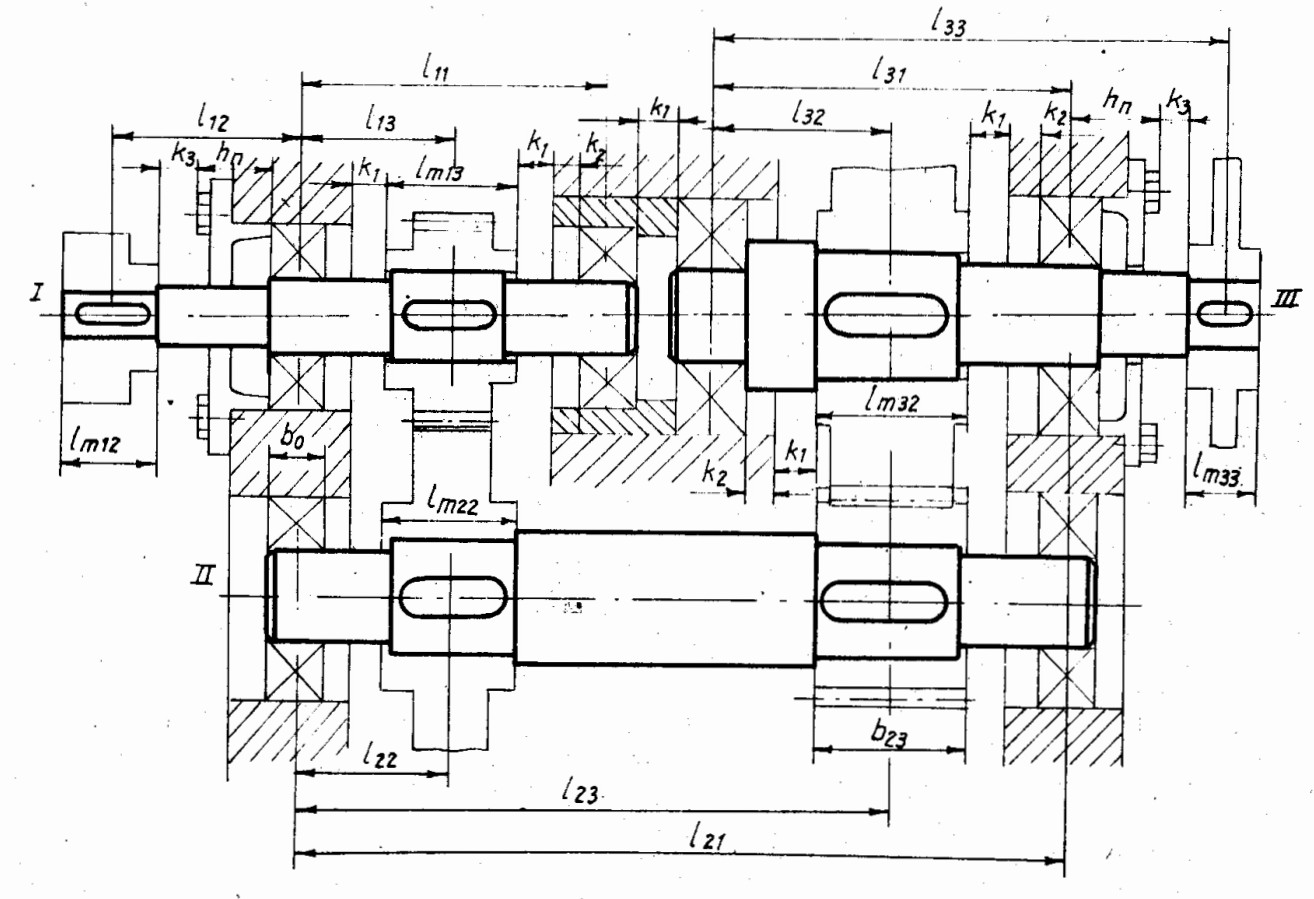
\includegraphics[width=150mm]{diagram}
	\caption{Dimensions and placement of 3 shafts in the speed reducer}
	\label{shaft}
\end{figure}

The gear widths are $ b_{12}=b_{21}=48.00\unit{mm} $ and $ b_{22}=b_{31} = 62.40\unit{mm}$, \textbf{Table \ref{chap4spec}} and \textbf{\ref{chap5spec}}. These values will be used to determine the minimum hub lengths $ l_{m13},l_{m22},l_{m32} $ (i.e. the hub length equals to shaft length at the gear mating section). Table 10.3 \cite{tk1} gives formulas to determine the necessary lengths in \textbf{Figure \ref{shaft}}. From design perspective, it is desirable to minimize the size of the speed reducer, thereby reducing material cost, bending moment and deflection of the shaft. This leads to the selection of hub lengths $ l_m $ shown below (refer to \textbf{Figure \ref{shaft}} for locating these dimensions):
\[
\begin{array}{l}
l_{m12} = 1.40 d_1 = 1.40\times 35 = 49 \unitp{mm}\\
l_{m13} = 1.20 d_1 = 1.20\times 35 = 42 \unitp{mm} \Rightarrow l_{m13} = 48.00 \unit{mm}\\
l_{m22} = 1.20 d_2 = 1.20\times 35 = 42 \unitp{mm} \Rightarrow l_{m13} = 48.00 \unit{mm}\\
l_{m32} = 1.20 d_3 = 1.20\times 45 = 54 \unitp{mm} \Rightarrow l_{m32} = 62.40 \unit{mm}\\
l_{m33} = 1.20 d_3 = 1.20\times 45 = 54 \unitp{mm} \Rightarrow l_{m33} = 67.50 \unit{mm}\\
\end{array}
\]

Equal spacing is better to reduce measuring time. Therefore, the lengths $ k_1, k_2, k_3, h_n $ are $ k_1 = 5 \unit{mm} $, $ k_2 = 5 \unit{mm} $, $ k_3 = 5 \unit{mm} $, $ h_n = 15 \unit{mm} $, where $ k_1 $ is the distance from the inner surface of the speed reducer to the nearer side of the mechanical drive and between mechanical drives,$ \unit{mm} $; $ k_2 $ is the distance from the inner surface of the bearings to the inner surface of the speed reducer,$ \unit{mm} $; $ k_3 $ is the distance from the bearing housing unit to the nearer side of the mechanical drive,$ \unit{mm} $; $ h_n $ is the vertical distance between the bearing housing unit and the screw head,$ \unit{mm} $. Then, the lengths in Table 10.4 \cite{tk1} for two-stage coaxial helical speed reducers are calculated as follows:

On shaft 1:
\begin{flalign*}
	l_{12} &= 0.5(l_{m12}+b_{O1})+k_3+h_n \\&= 0.5(49 + 21)+5+5 = 55.00\unitp{mm}\\
	l_{13} &= 0.5(l_{m13}+b_{O1})+k_1+k_2 \\&= 0.5(48.00 + 21)+ 8+ 5 = 44.50\unitp{mm}\\
	l_{11} &= 2l_{13} = 2\times 44.50 = 89.00\unitp{mm}\\
\end{flalign*}

On shaft 3:
\begin{flalign*}
	l_{32} &= 0.5(l_{m32}+b_{O3})+k_1+k_2 \\&= 0.5(62.40 + 25)+ 5 + 5 = 54.00\unitp{mm}\\
	l_{31} &= 2l_{32} = 2\times 54.00 = 108.00\unitp{mm} \\
	l_{33} &= l_{31} + 0.5(l_{m33}+b_{O3})+k_3+h_n \\ & = 108.00 + 0.5(67.50 + 25) + 5 + 15 = 174.25\unitp{mm} \Rightarrow l_{33} = 175\unit{mm}
\end{flalign*}

On shaft 2:
\begin{flalign*}
	l_{22} &= 0.5(l_{m22}+b_{O2})+k_1+k_2 \\&= 0.5(48.00 + 21) + 5 + 5  = 44.50 \unitp{mm}\\
	l_{23} &= l_{11}+l_{32}+k_1+0.5(b_{O1}+b_{O3}) \\&= 89.00+54.00+5+0.5(21+25) = 171.00 \unitp{mm}\\
	l_{21} &= l_{23}+l_{32} = 171.00+54.00 = 225.00\unitp{mm}
\end{flalign*}

\subsection{Find reaction forces}
The speed reducer operates at constant speed. Therefore, the equilibrium conditions are
\[
\left\{ 
\begin{array}{l@{{}={}}l}
\displaystyle\sum_{i} \mathbf{F_{i}} & 0\\
\displaystyle\sum_{i} \mathbf{r_i}\times \mathbf{F_i}& 0\\
\end{array}
\right.
\]

The equations above are applied to 3 pairs of bearings, each of which is mounted on 1 shaft. Projecting the forces onto 2 planes $ Oxy $ and $ Oyz $ yields 6 sets of matrices in the form of $ AX + B = 0 $ where $ X $ is the $ 2\times 1 $ matrix whose unit is$ \unit{N} $. The solutions are shown in \textbf{Table \ref{soltab}}:

\begin{table}
	\centering
	\caption{Tabularized equations for reaction forces in matrix form}
		\begin{tabular}{llll}\toprule
		$ A $  & $ X \unitp{N} $  & $ B $ & $X=A^{-1}(-B) $  \\\midrule\addlinespace[1.5ex]
		$ \begin{bmatrix} 1 & 1\\ l_{12} & l_{12}+l_{11} \end{bmatrix}  $  & 
		$ \begin{bmatrix} F_{1Bx}\\ F_{1Dx} \end{bmatrix} $ & 
		$ \begin{bmatrix} F_{12x}\\ (l_{12}+l_{13})F_{12x}+0.5d_{12}F_{12z} \end{bmatrix} $ &
		$ \begin{bmatrix} -555.53\\ -103.6 \end{bmatrix} $\\\addlinespace[1.5ex]
		$ \begin{bmatrix} 1 & 1\\ l_{12} & l_{12}+l_{11} \end{bmatrix}  $  & 
		$ \begin{bmatrix} F_{1By}\\ F_{1Dy} \end{bmatrix} $ & 
		$ \begin{bmatrix} F_{12y}\\ (l_{12}+l_{13})F_{12y} \end{bmatrix} $ &
		$ \begin{bmatrix} -555.53\\ -308.52 \end{bmatrix} $\\\addlinespace[1.5ex]
		$ \begin{bmatrix} 1 & 1\\ 0 & l_{21} \end{bmatrix}  $  & 
		$ \begin{bmatrix} F_{2Ax}\\ F_{2Dx} \end{bmatrix} $ & 
		$ \begin{bmatrix} F_{21x}+F_{22x}\\ l_{22}F_{21x}+l_{23}F_{22x}+0.5d_{21}F_{21z}+0.5d_{22}F_{22z} \end{bmatrix} $ &
		$ \begin{bmatrix} 1159.54\\ 71.7 \end{bmatrix} $\\\addlinespace[1.5ex]
		$ \begin{bmatrix} 1 & 1\\ 0 & l_{21} \end{bmatrix}  $  & 
		$ \begin{bmatrix} F_{2Ay}\\ F_{2Dy} \end{bmatrix} $ & 
		$ \begin{bmatrix} F_{21y}+F_{22y}\\ l_{22}F_{21y}+l_{23}F_{22y} \end{bmatrix} $ &
		$ \begin{bmatrix} 1069.12 \\ -792.77 \end{bmatrix} $\\\addlinespace[1.5ex]
		$ \begin{bmatrix} 1 & 1\\ 0 & l_{31} \end{bmatrix}  $  & 
		$ \begin{bmatrix} F_{3Ax}\\ F_{3Cx} \end{bmatrix} $ & 
		$ \begin{bmatrix} F_{31x}+F_{32x}\\ l_{32}F_{31x}+l_{33}F_{32x}+0.5d_{31}F_{31z} \end{bmatrix} $ &
		$ \begin{bmatrix} 1762 \\ -192.23 \end{bmatrix} $\\\addlinespace[1.5ex]
		$ \begin{bmatrix} 1 & 1\\ 0 & l_{31} \end{bmatrix}  $  & 
		$ \begin{bmatrix} F_{3Ay}\\ F_{3Cy} \end{bmatrix} $ & 
		$ \begin{bmatrix} F_{31y}+F_{32y}\\ l_{32}F_{31y}+l_{33}F_{32y} \end{bmatrix} $ &
		$ \begin{bmatrix} -6620.6\\ 1325.42 \end{bmatrix} $\\\addlinespace[1.5ex]
		\bottomrule
	\end{tabular}
	\label{soltab}
\end{table}

For convenience, the values of variables in \textbf{Table \ref{soltab}} are mentioned here:

Dimension values:
\[
\begin{array}{l}
l_{11} = 89.00\unit{mm}, l_{12} = 44.50\unit{mm}, l_{13} = 55.00\unit{mm}\\
l_{21} = 225.00\unit{mm}, l_{22} = 44.50\unit{mm}, l_{23} = 171.00\unit{mm}\\
l_{31} = 108.00\unit{mm}, l_{32} = 54.00\unit{mm}, l_{33} = 175.00\unit{mm}\\
d_{12} = 83.57\unit{mm}, d_{21} = 236.43\unit{mm}, d_{22} = 83.08\unit{mm}, d_{31} = 236.92\unit{mm}
\end{array}
\]

Force values:
\[
\begin{array}{l}
F_{12} = \begin{bmatrix} F_{12x} & F_{12y} & F_{12z}\end{bmatrix} = \begin{bmatrix} -1111.06 & -412.12 & -218.24\end{bmatrix} \unit{N}\\
F_{21} = \begin{bmatrix} F_{21x} & F_{21y} & F_{21z}\end{bmatrix} = \begin{bmatrix} 1111.06 & 412.12 & 218.24\end{bmatrix} \unit{N}\\
F_{22} = \begin{bmatrix} F_{22x} & F_{22y} & F_{22z}\end{bmatrix} = \begin{bmatrix} 1117.61 & -1133.19 & -691.82\end{bmatrix} \unit{N}\\
F_{31} = \begin{bmatrix} F_{31x} & F_{31y} & F_{31z}\end{bmatrix} = \begin{bmatrix} -1117.61 & 1133.19 & 691.82 \end{bmatrix} \unit{N}\\
F_{32} = \begin{bmatrix} F_{32x} & F_{32y} & F_{32z}\end{bmatrix} = \begin{bmatrix} 3741 & 0 & 0 \end{bmatrix} \unit{N}\\
\end{array}
\]

From the reaction forces, the shear force diagrams for 3 shafts are created but will not be shown. From the shear force diagrams, the bending moment diagrams for 3 shafts are visualized as demonstrated in Fi\textbf{gure \ref{mshaft1}}, \textbf{\ref{mshaft2}} and \textbf{\ref{mshaft3}}. The moments at critical sections are computed below:\\
Shaft 1, $ Oxz $-plane:
\[
\begin{array}{l}
M_{1Ax} = 0 \unitp{N\cdot mm}\\
M_{1Bx} = l_{12}F_{1By} = -5698.14 \unitp{N\cdot mm}\\
M_{1Cx}^- = l_{12}F_{1By}+(l_{12}+l_{13})F_{12y} = 35307.65 \unitp{N\cdot mm}\\
M_{1Cx}^+ = l_{12}F_{1By}+(l_{12}+l_{13})F_{12y}+d_{12}/2\times F_{21z} = 44426.31 \unitp{N\cdot mm}\\
M_{1Dx} = 0 \unitp{N\cdot mm}\\
\end{array}
\]
Shaft 1, $ Oyz $-plane:
\[
\begin{array}{l}
M_{1Ay} = 0 \unitp{N\cdot mm}\\
M_{1By} = l_{12}F_{1Bx} = -30554.04 \unitp{N\cdot mm}\\
M_{1Cy} = l_{12}F_{1Bx}+(l_{12}+l_{13})F_{21x} = 79996.02 \unitp{N\cdot mm}\\
M_{1Dy} = 0 \unitp{N\cdot mm}
\end{array}
\]
Shaft 2, $ Oxz $-plane:
\[
\begin{array}{l}
M_{2Ax} = 0 \unitp{N\cdot mm}\\
M_{2Bx}^- = l_{22}F_{12y} =  -18339.27 \unitp{N\cdot mm}\\
M_{2Bx}^+ = l_{22}F_{12y} + d_{21}/2\times F_{12z} = -44138.39 \unitp{N\cdot mm}\\
M_{2Cx}^- = l_{22}F_{12y} + l_{23}F_{31y} + d_{21}/2\times F_{12z} = 149637.15 \unitp{N\cdot mm}\\
M_{2Cx}^+ = l_{22}F_{12y} + l_{23}F_{31y} + d_{21}/2\times F_{12z} + d_{22}/2\times F_{31z} = 178374.12 \unitp{N\cdot mm}\\
M_{2Dx} = 0 \unitp{N\cdot mm}\\
\end{array}
\]
Shaft 2, $ Oyz $-plane:
\[
\begin{array}{l}
M_{2Ay} = 0 \unitp{N\cdot mm}\\
M_{2By} = l_{22}F_{1Bx} = -49441.98 \unitp{N\cdot mm}\\
M_{2Cy} = l_{22}F_{1Bx}+(l_{12}+l_{13})F_{12x} = -240553.02 \unitp{N\cdot mm}\\
M_{2Dy} = 0 \unitp{N\cdot mm}
\end{array}
\]
Shaft 3, $ Oxz $-plane:
\[
\begin{array}{l}
M_{3Ax} = 0 \unitp{N\cdot mm}\\
M_{3Bx}^- = l_{32}F_{22y} = -61192.27 \unitp{N\cdot mm}\\
M_{3Bx}^+ = l_{32}F_{22y}+d_{31}/2\times F_{22z} = -143145.85 \unitp{N\cdot mm}\\
M_{3Cx} = l_{32}F_{22y}+l_{31}F_{3By}+d_{31}/2\times F_{22z} = 0 \unitp{N\cdot mm}\\
M_{3Dx} = 0 \unitp{N\cdot mm}\\
\end{array}
\]
Shaft 3, $ Oxz $-plane:
\[
\begin{array}{l}
M_{3Ay} = 0 \unitp{N\cdot mm}\\
M_{3By} = l_{32}F_{22x} = 60350.85 \unitp{N\cdot mm}\\
M_{3Cy} = l_{32}F_{22x}+l_{31}F_{3Bx} = -654674.15 \unitp{N\cdot mm}\\
M_{3Dy} = 0 \unitp{N\cdot mm}
\end{array}
\]

After computing all bending moments at critical sections, Equation 10.17 \cite{tk1} is used to estimate minimum diameter $ d_{est} $ at a cross section corresponding to the magnitude of moments there. The values are summarized in col. 6, \textbf{Table \ref{dia_sh}}:
\[
d_{est} = \sqrt[3]{\dfrac{10M_e}{[\sigma]}}
\]
where
\begin{itemize}
	\item $ M_e $ is the equivalent bending moment including the input torque. It is calculated using Equation 10.16, \cite{tk1}. The values of $ M_e $ at each critical cross section are shown in col. 5, \textbf{Table \ref{dia_sh}}:
	\[
	M_e = \sqrt{M_x^2 + M_y^2 + 0.75T_{sh}}
	\]
	where
	\begin{itemize}
		\item $ M_x $ is the bending moment on $ Oxz $ plane, calculated above.
		\item $ M_y $ is the bending moment on $ Oyz $ plane, calculated above.
		\item $ T_{sh} $ is the input torque from the motor,$ \unit{N\cdot mm} $. The values are given in \textbf{Table \ref{tab:my-table}}.
	\end{itemize}
	\item $ [\sigma] $ is the permissible stress of shaft material, Table 10.5 \cite{tk1}. In this design project, all 3 shafts are fabricated from the same material (carbon steel AISI 1035) yielding at $ \sigma_b = 586\unit{MPa} $ (ultimate strength).
\end{itemize}

The selection of suitable diameters depends not only on stress condition but also the geometry of the shaft itself (i.e. mechanical drives are mounted in clearance, transition or interference fit and does not collide with the shaft). Therefore, during calculation, at cross sections where moment jump occurs, Equation 10.17 \cite{tk1} yields 2 minimum diameters. In such cases, the larger value is selected. In addition, at cross sections where the total bending moment is 0, the minimal diameter $ d_{est} $ determined by Equation 10.17 \cite{tk1} is incorrect. Thus it is best to relate to adjoining diameters and choose according to standard. From \textbf{Table \ref{dia_sh}}, the cross sections with zero equivalent bending moment are
\begin{itemize}
	\item shaft 1: $ M_{1D} $. The choice of $ d_{1D} $ is determined by the value of $ d_{1B} $ since a pair of bearings is mounted on sections $ B $ and $ D $.
	\item shaft 2: $ M_{2A}, M_{2D} $. A pair of bearings is mounted on sections $ A $ and $ D $, which makes the approach from shaft 1 unreasonable. Hence, $ d_{2A}, d_{2D} $ are chosen so that they are not too small with respect to either $ d_{2B} $ or $ d_{2C} $ while still following the standard.
	\item shaft 3: $ M_{3A} $. Similar to shaft 1, the diameter at $ A $ equals to that at $ C $ since a pair of bearings is mounted there.
\end{itemize}

\begin{table}[ht]
	\centering
	\caption{Equivalent moment $ M_e $ and cross section diameters of 3 shafts}
	\begin{tabular}{lllllll}\toprule
		Sect. & $ M_x\unitp{N\cdot mm} $  & $ M_y\unitp{N\cdot mm} $ & $ T_{sh}\unitp{N\cdot mm} $ & $ M_e\unitp{N\cdot mm} $ & $ d_{est}\unitp{mm} $ & $ d\unitp{mm} $ \\ \midrule
		$ 1A $		&	0			&	0			&	46423.73	& 40204.13	&	20.12	& 32 \\
		$ 1B $		&	-5698.14	&	-30554.04	&	46423.73	& 50817.22	&	21.76	& 35 \\
		$ 1C^- $	&	35307.65	&	79996.02	&	46423.73	& 96241.19	&	26.92	& 42 \\
		$ 1C^+ $	&	44426.31	&	79996.02	&	0			& 91504.43	&	26.47	& 42 \\
		$ 1D $		&	0			&	0			&	0			& 0			&	0		& 35 \\
		$ 2A $		&	0			&	0			&	0			& 0			&	0		& 45 \\
		$ 2B^- $	&	-18339.27	&	-49441.98	&	0			& 52733.66	&	23.3	& 54 \\
		$ 2B^+ $	&	-44138.39	&	-49441.98	&	126093.3	& 127739.37	&	31.29	& 54 \\
		$ 2C^- $	&	149637.15	&	-240553.02	&	126093.3	& 303614.35	&	41.76	& 54 \\
		$ 2C^+ $	&	178374.12	&	-240553.02	&	0			& 299471.34	&	41.57	& 54 \\
		$ 2D $		&	0			&	0			&	0			& 0			&	0		& 45 \\
		$ 3A $		&	0			&	0			&	0			& 0			&	0		& 60 \\
		$ 3B^- $	&	-61192.27	&	60350.85	&	0			& 85946.03	&	26.75	& 69 \\
		$ 3B^+ $	&	-143145.85	&	60350.85	&	342486.86	& 334822.19	&	42.09	& 69 \\
		$ 3C $		&	0			&	-654674.15	&	342486.86	& 718728.86	&	54.3	& 60 \\
		$ 3D $		&	0			&	0			&	342486.86	& 296602.32	&	40.43	& 52 \\
		\bottomrule
	\end{tabular}
	\label{dia_sh}
\end{table}

\begin{figure}[ht]
	\centering
	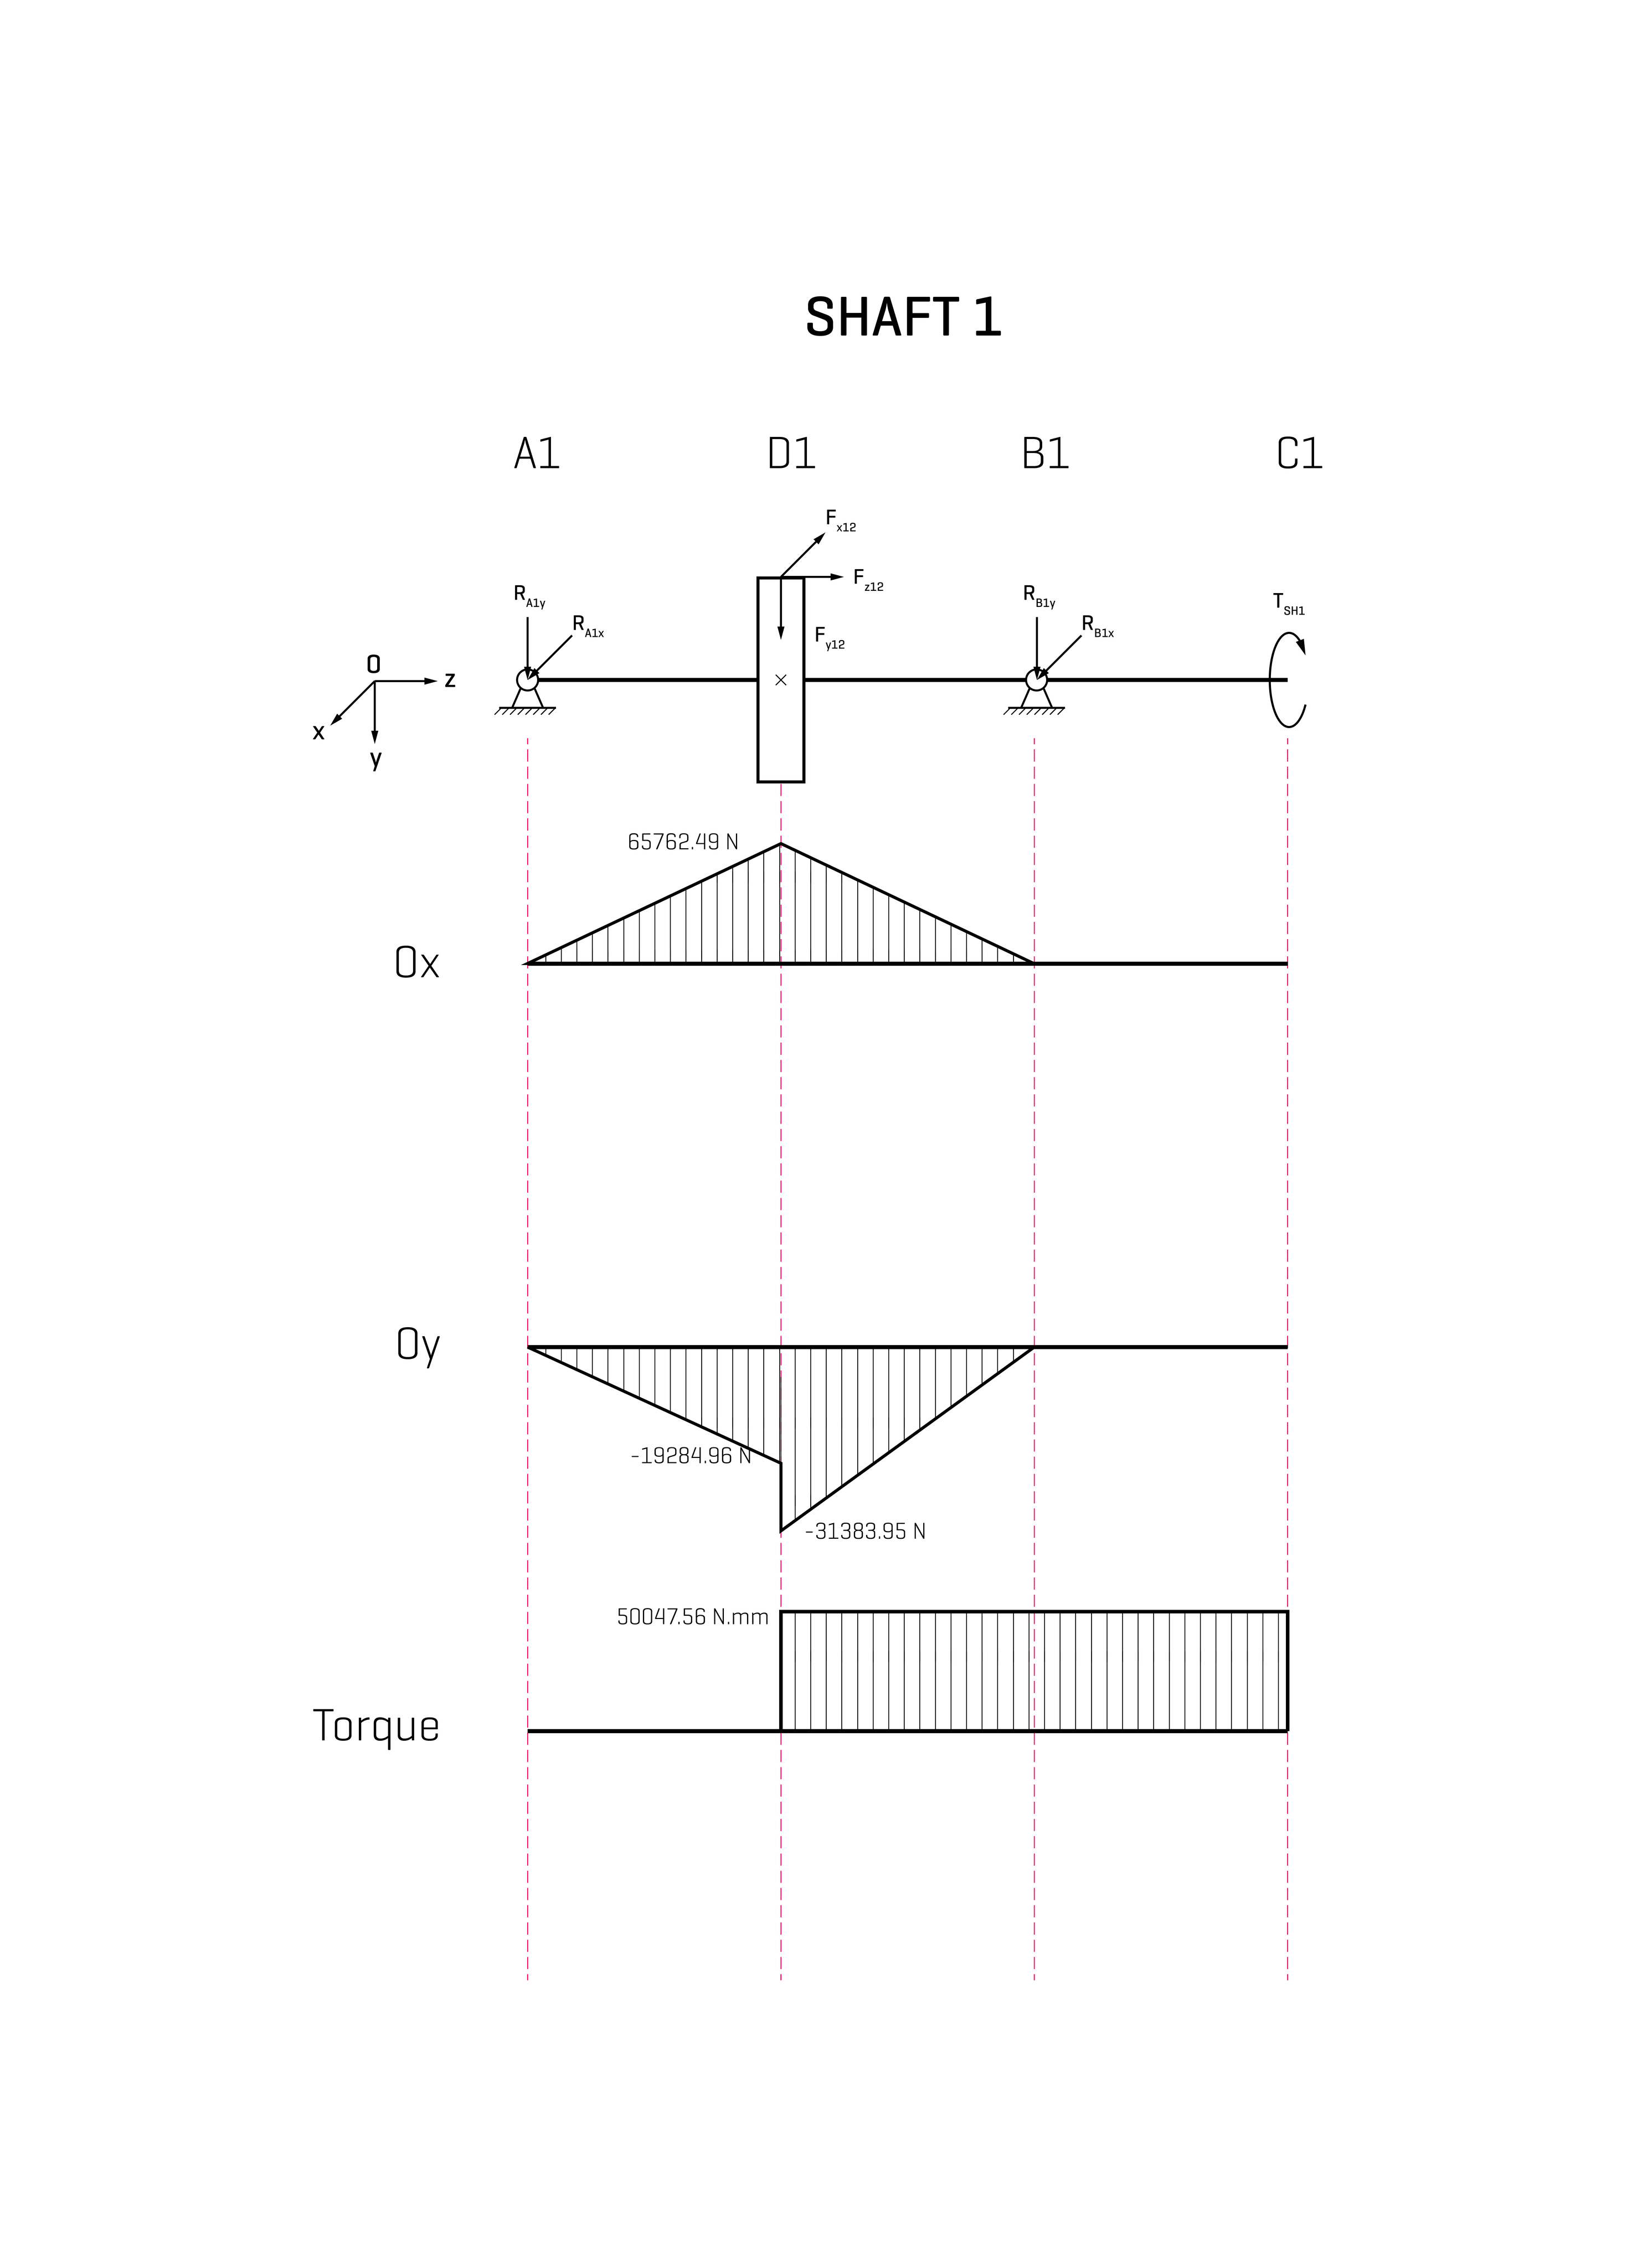
\includegraphics[width=0.8\linewidth]{mshaft1}
	\caption{Bending moment-torque diagram and section view of shaft 1}
	\label{mshaft1}
\end{figure}

\begin{figure}[ht]
	\centering
	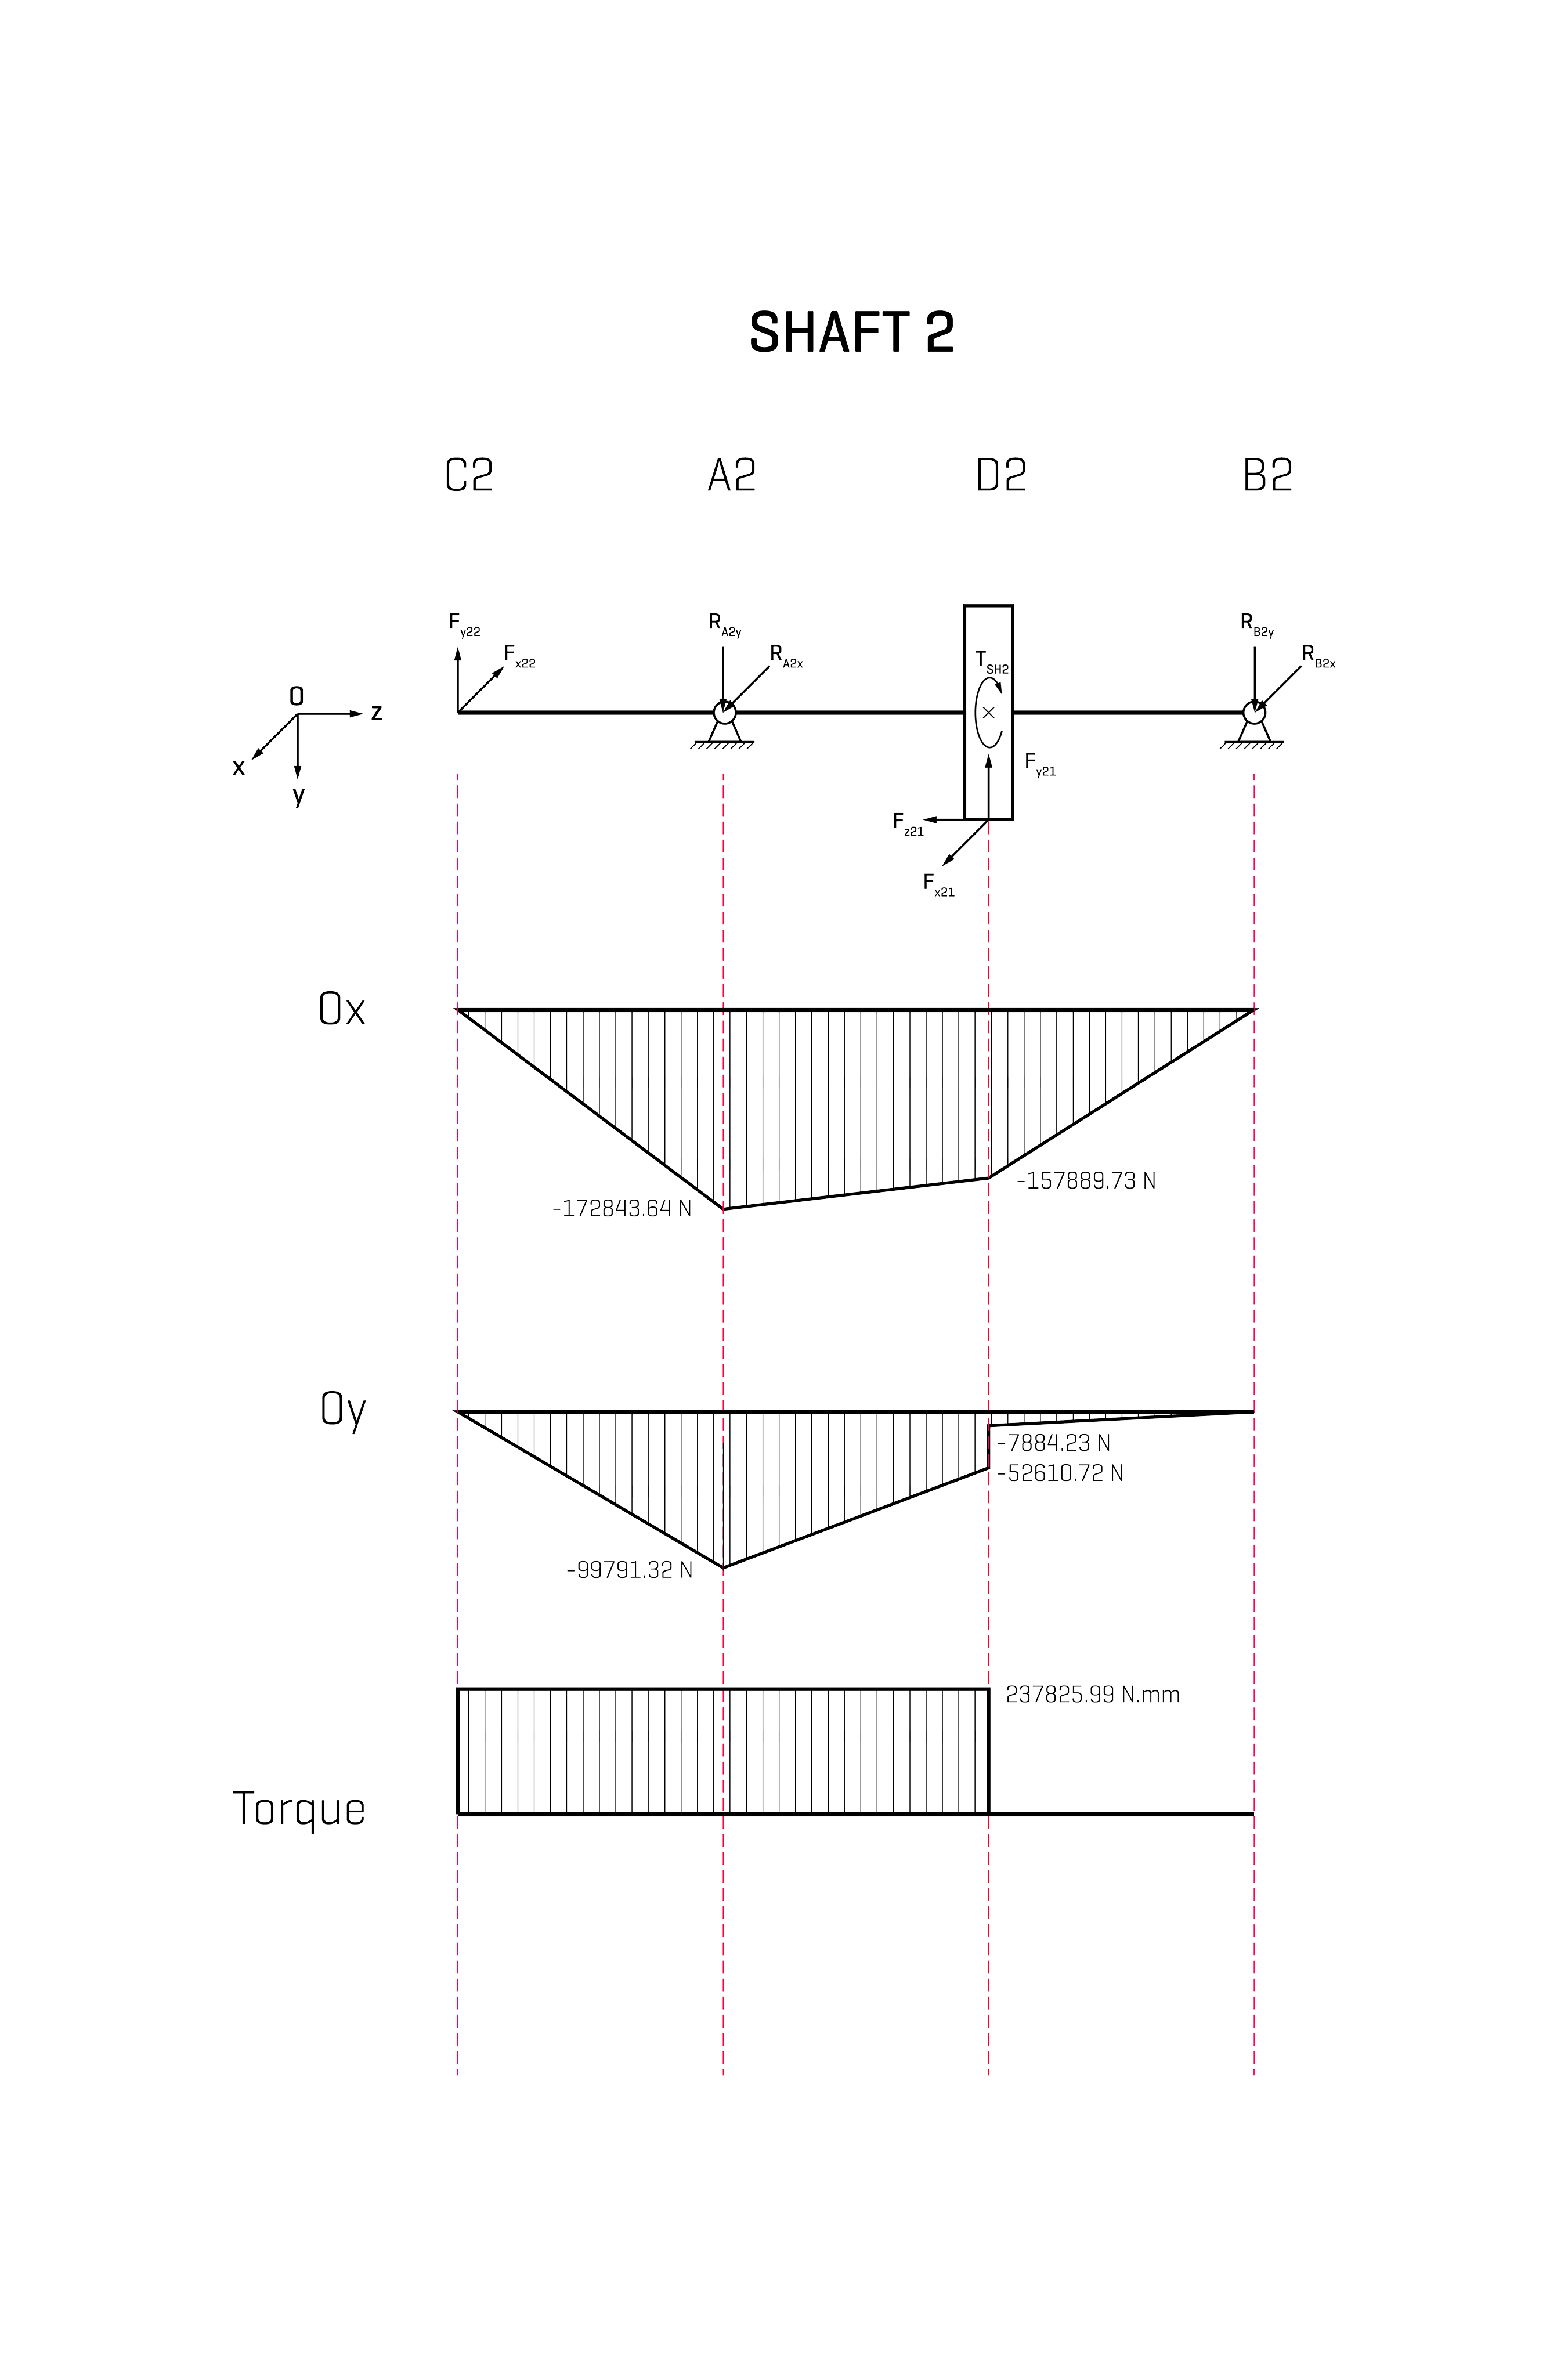
\includegraphics[width=\linewidth]{mshaft2}
	\caption{Bending moment-torque diagram and section view of shaft 2}
	\label{mshaft2}
\end{figure}

\begin{figure}[ht]
	\centering
	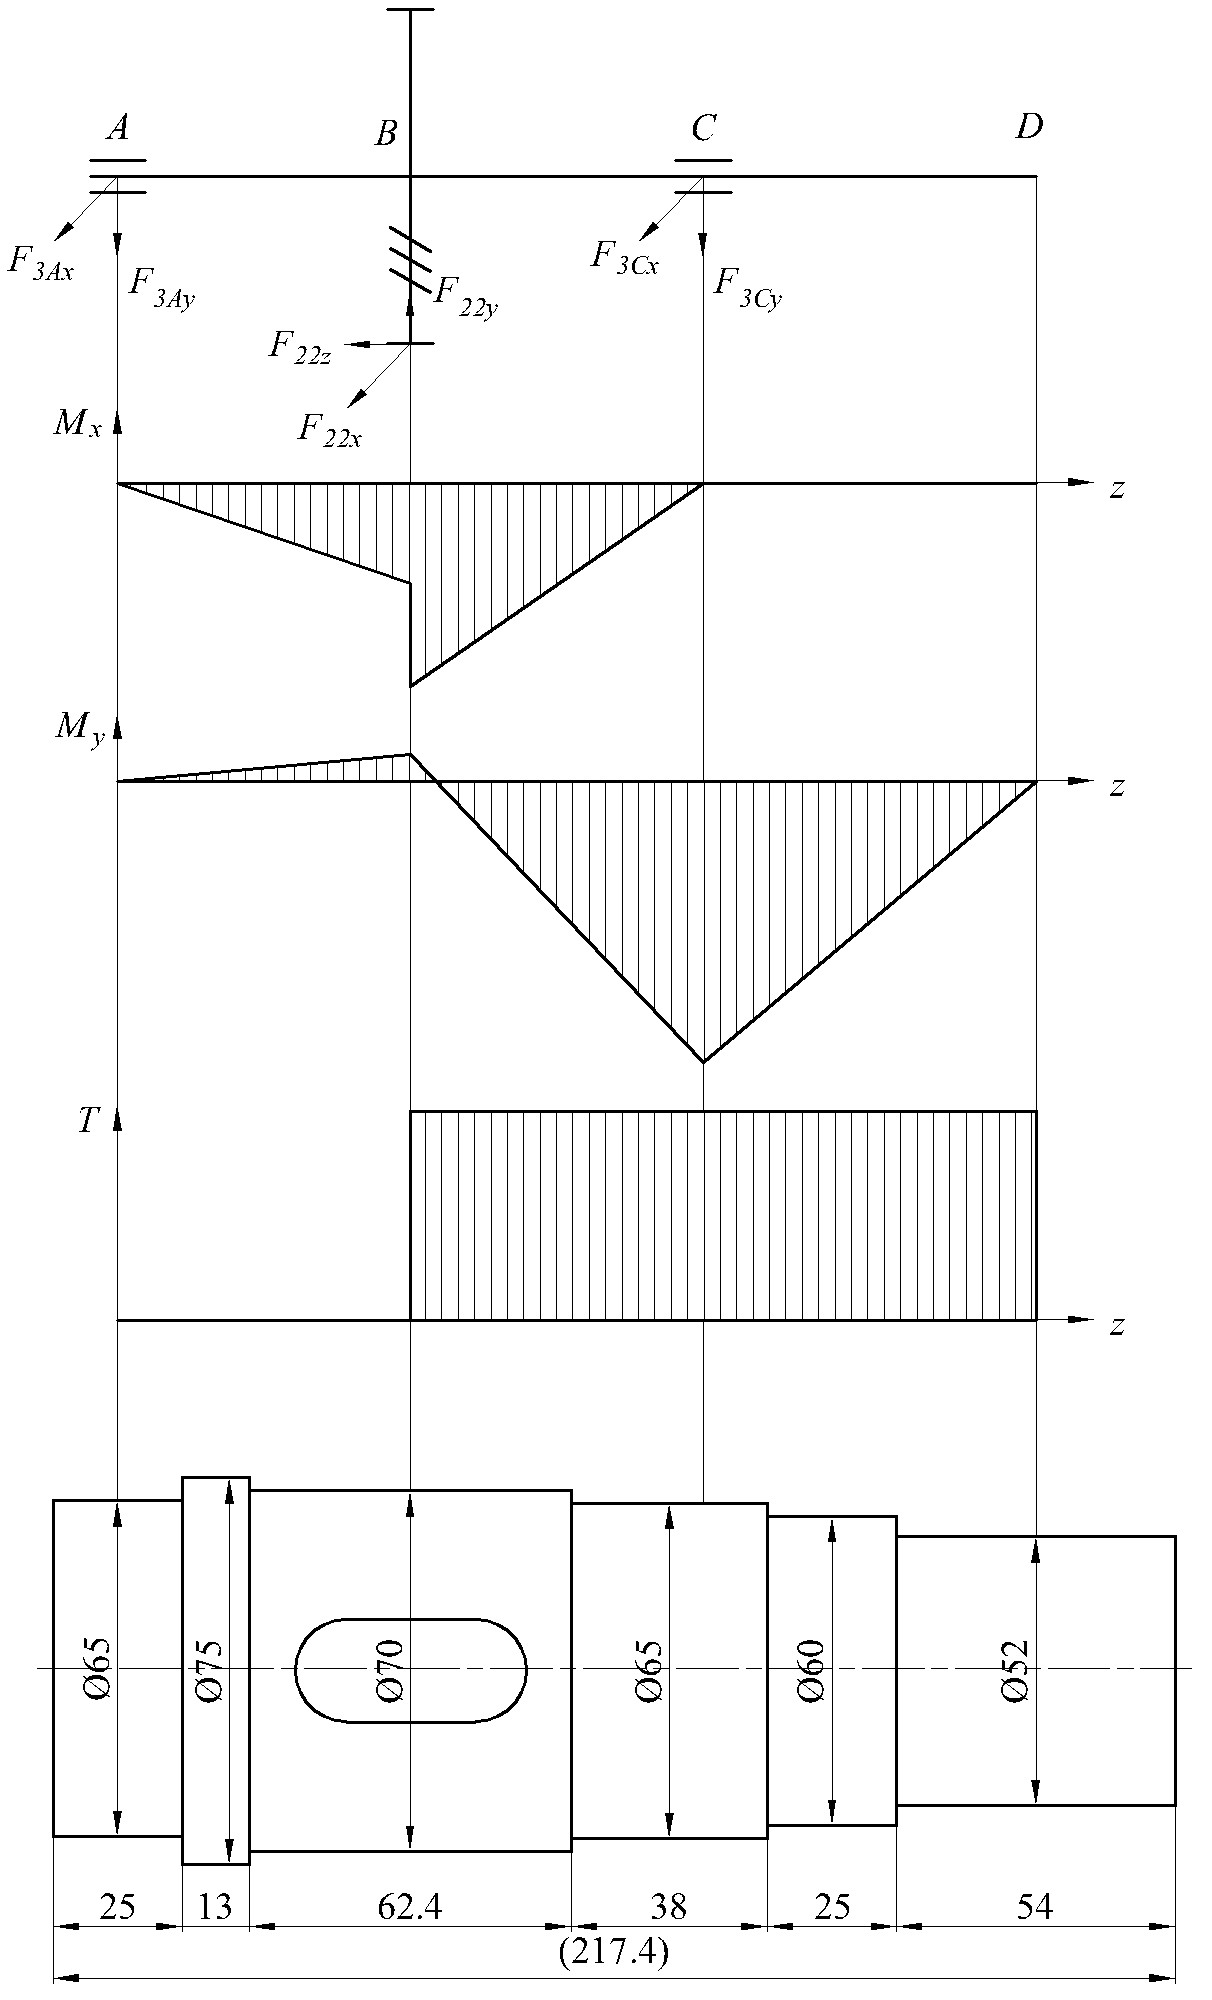
\includegraphics[width=0.8\linewidth]{mshaft3}
	\caption{Bending moment-torque diagram and section view of shaft 3}
	\label{mshaft3}
\end{figure}

In addition, the geometry of the shafts requires modification. Each shaft has 4 cross sections with diameter alteration. The purpose is to mount and fix the gear(s) with keys. Therefore, from Figure 1.2,
\begin{itemize}
	\item on shaft 1 (designated I in the figure): diameter 2 starting from the left of the shaft must be smaller than the bearing diameter $ d_{1B} $ so that the bearing from the left can be slid right into the shaft (i.e. $ d_{1A} = 32 \unit{mm} < d{1AB} < d_{1B} = 35 \unit{mm} $). Thus, choosing from standard on p.195 \cite{tk1}, the diameter is $ d_{1AB} = 34 \unit{mm} $.
	\item on shaft 2 (designated II in the figure): diameter 3 starting from the left of the shaft must be larger than bore diameter of the 2 mounted gears. In that way, both gears can be supported from 1 end (i.e. prevent sliding on 1 direction). The range for selecting diameter 3 is $ d_{2BC} \geq \max(d_{2B}, d_{2C}) = 54 \unit{mm} $. Choosing from standard on p.195 \cite{tk1}, the diameter is $ d_{2BC} = 60 \unit{mm} $.
	\item on shaft 3 (designated III in the figure): diameter 2 starting from the left of the shaft must be larger than $ d_{3B} = 69 \unit{mm} $ to support the gear from 1 end. Choosing from standard on p.195 \cite{tk1}, the diameter is $ d_{3AB} = 84 \unit{mm} $.
\end{itemize}
\clearpage

\section{Design of keys and keyways}
\subsection{Calculate key dimensions}

Fixation of mechanical drives for power transmission purpose requires keys. For simple applications, parallel key is good enough. The dimensions of parallel keys are specified in \textbf{Figure \ref{keydim}}.

\begin{figure}[ht]
	\centering
	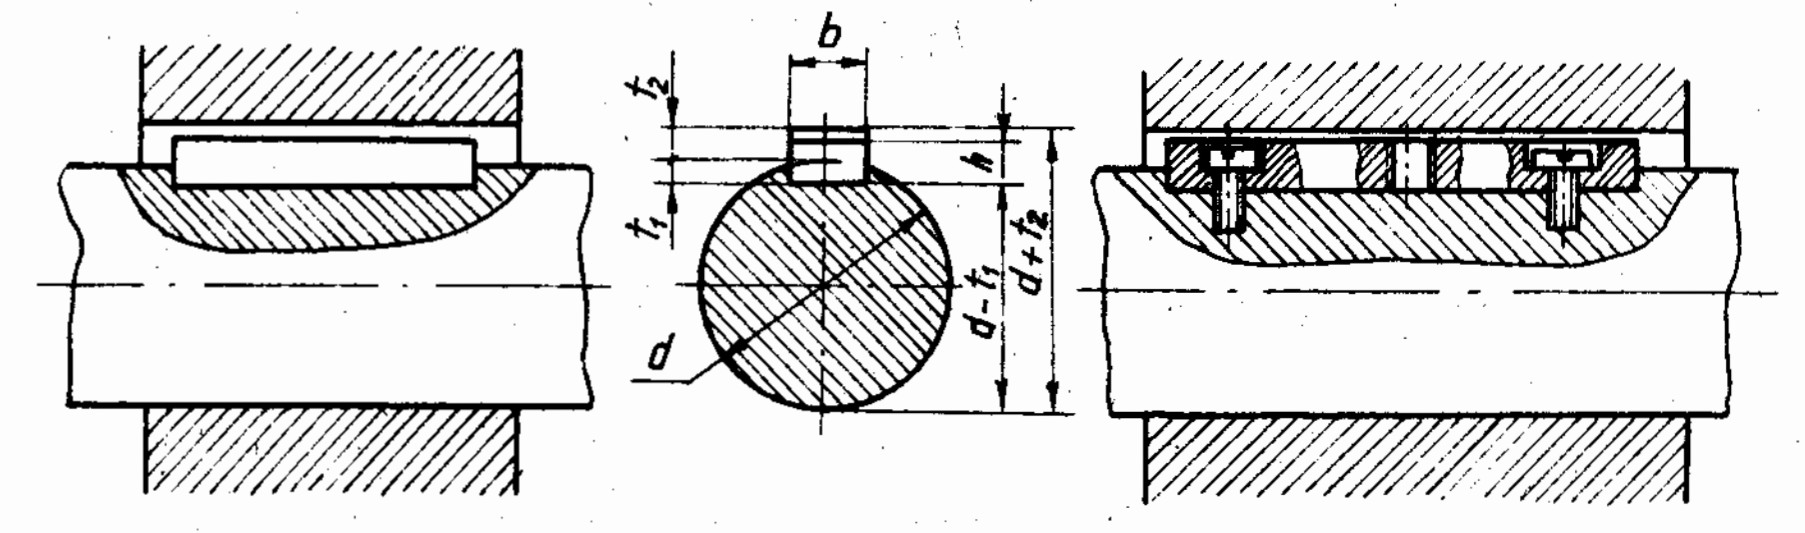
\includegraphics{keydim}
	\caption{Key dimensions according to Vietnam Standard TCVN 2261-77}
	\label{keydim}
\end{figure}

Choosing key dimension according to standard yields (Table 9.1a \cite{tk1}):

\begin{table}[ht]
	\centering
	\caption{Selection of key dimensions (all units are in$ \unit{mm} $)}
	\begin{tabular}{lllllll}\toprule
		Sect. & $ d $ & $ b $ & $ h $ & $ t_1 $ & $ t_2 $ & $ l $\\\midrule
		$ 1A $ & 32 & 10 & 8 & 5 & 3.3 & 32\\
		$ 1C $ & 42 & 10 & 8 & 5 & 3.3 & 32\\
		$ 2B $ & 54 & 16 & 10 & 6 & 4.3 & 32\\
		$ 2C $ & 54 & 16 & 10 & 6 & 4.3 & 45\\
		$ 3B $ & 69 & 18 & 11 & 7 & 4.4 & 45\\
		$ 3D $ & 52 & 16 & 10 & 6 & 4.3 & 35\\\bottomrule
	\end{tabular}
	\label{keydimtab}
\end{table}

After determining the dimensions, the edge of these keys are chamferred $ 0.4\times 0.4 \unit{mm} $ to reduce stress concentration factor accumulated in sharp corners. For this reason, the edge of the keyways are machined into fillet radius $ r = 0.4 \unit{mm} $.

\subsection{Stress analysis of key}
The stress analysis of keys are determined by Equation 9.1 and 9.2 \cite{tk1}:
\[
\begin{array}{l}
\sigma_d = 2T/[(dl(h-t_1))] \leq [\sigma_d]\\
\tau_c = 2T/(dlb) \leq [\tau_c]
\end{array}
\]
where
\begin{itemize}
	\item $ \sigma_d $ is the compressive stress exerting on the key,$ \unit{MPa} $.
	\item $ T $ is the applied torque onto the shaft. The torque $ T_{sh1} $, $ T_{sh2} $, $ T_{sh3} $ exert on shaft 1, 2, 3, respectively. The numerical values are given in \textbf{Table \ref{tab:my-table}}.
	\item $ d $ is the diameter of shaft at the cross section,$ \unit{mm} $. The value is given in \textbf{Table \ref{dia_sh}}.
	\item $ l, h, t_1, b $ are key dimensions. The values are provided in \textbf{Table \ref{keydimtab}}.
	\item $ [\sigma_d] $ is the permissible compressive stress,$ \unit{MPa} $. The value is provided in Table 9.5 \ref{tk1}. The gear is made of carbon steel, load condition is light impact and the assembly is fixed. This configuration corresponds to $ [\sigma_d] = 100 \unit{MPa} $
	\item $ \tau_c $ is the torsion stress exerting on the key,$ \unit{MPa} $.
	\item $ [\tau_c] $ is the permissible torsion stress exerting on the key,$ \unit{MPa} $. For light impact load, $ [\tau_c] = 40 \unit{MPa} $.
\end{itemize}

The results are summarized in \textbf{Table \ref{keystress}}.
\begin{table}[ht]
	\centering
	\caption{Stress analysis of keys}
	\begin{tabular}{llllllllll}\toprule
		Sect. & $ T $ & $ d $ & $ l $ & $ h $ & $ t_1 $ & $ b $ & $ \sigma_d $ & $ \tau_c $\\\midrule
		$ 1A $ & 46423.73 & 32 & 32 & 8  & 5 & 10 & 30.22 & 9.07 \\
		$ 1C $ & 46423.73 & 42 & 32 & 8  & 5 & 10 & 23.03 & 5.76 \\
		$ 2B $ & 126093.3 & 54 & 32 & 10 & 6 & 16 & 36.49 & 9.12 \\
		$ 2C $ & 126093.3 & 54 & 45 & 10 & 6 & 16 & 25.95 & 6.49 \\
		$ 3B $ & 342486.86& 69 & 45 & 11 & 7 & 18 & 41.36 & 12.26 \\
		$ 3D $ & 342486.86& 52 & 35 & 10 & 6 & 16 & 70.57 & 23.52 \\\bottomrule
	\end{tabular}
	\label{keystress}
\end{table}

\section{Strength of the shafts}
\subsection{Fatigue Strength Analysis}
For each critical section, the fatigue strength safety factor there must satisfy this condition:
\[s=\dfrac{s_\sigma s_\tau}{\sqrt{s_\sigma^2+s_\tau^2}}\geq[s]\]
where
\begin{itemize}
	\item $ [s] $ is the permissible fatigue strength at a cross section. If $ [s]>2.5 $, deflection analysis can be ignored.
	\item $ s_\sigma $ is the tensile stress safety factor at a cross section. It is computed using Inequation 10.20 \cite{tk1}:
	\[
	s_\sigma = \dfrac{\sigma_{-1}}{K_\sigma\sigma_a + \psi_\sigma\sigma_m}
	\]
	where
	\begin{itemize}
		\item $ \sigma_{-1} $ is the permissible bending fatigue stress in a cycle,$ \unit{MPa} $. For carbon steel, it is estimated using equation:
		\[
		\sigma_{-1} = 0.436\sigma_b
		\]
		where $ \sigma_b $ is the yielding stress of material,$ \unit{MPa} $. All 3 shafts use the same material, which is C35 steel. Therefore, and $ \sigma_{-1} = 0.436\times 585 = 255.06\unit{MPa} $.
		\item $ K_\sigma $ is the overall factor regarding tension stress at a cross section. It is computed using Equation 10.25 \cite{tk1}:
		\[
		K_\sigma = \dfrac{k_\sigma/\varepsilon_\sigma + K_x - 1}{K_y}
		\]
		where
		\begin{itemize}
			\item $ k_\sigma $ is the stress concentration factor due to bending stress, Table 10.13 \cite{tk1}. The factor depends on geometry of shoulder fillets. Although various techniques have been developed (undercut, inserted ring, undercut to simulate a ring, relief groove, etc.), for simplicity, corner radius method is used only.
			
			It is recommended that the fillet radius be as large as possible to minimize $ k_\sigma $, However, the design of the gear, bearing, or other element affects the radius that can be used, p.517 \cite{mott_vavrek_wang_2018}. Therefore, at cross sections where diameter changes, the fillet radius $ r $ is computed using the ratio $ r/d = 0.5(D-d) $, where $ D $ is the larger diameter and $ d $ is the smaller diameter. In areas where parts are mounted to the shaft, the ratio is $ r/d \leq 0.02 $. The reason is to avoid collision between the part and the shaft if the part is not filleted around its edge. In case of shaft 1, those parts are coupling and bearings; for shaft 2, they are bearings; for shaft 3, they are bearings and driving sprocket of the chain drive.
			\item $ \varepsilon_\sigma $ is the size factor corresponding to bending stress, Table 10.10 \cite{tk1}. The factor depends on the choice of material, which in this case is carbon steel for all 3 shafts.
			\item $ K_x $ is the stress concentration factor due to surface finishing, Table 10.8 \cite{tk1}. For all 3 shafts, the surface is lathed roughly for assembly and cost reduction purpose. Thus, $ K_x = 1.2 $
			\item $ K_y $ is the strengthening factor. It is unnecessary to harden the surface since the diameters of all 3 shafts are sufficiently larger than their minimal values, col. 6 and 7, \textbf{Table \ref{dia_sh}}. $ K_y = 1 $
		\end{itemize}
		\item $ \sigma_a $ is the amplitude of bending stress in a cycle. For rotating shaft, which are all 3 shafts, it is computed using Equation 10.22 \cite{tk1}:
		\[ \sigma_a = \sqrt{M_x^2 + M_y^2}/W \]
		where $ M_x $ is the moment about $ x $-axis; $ M_y $ is the moment about $ y $-axis; $ W $ is the shaft volume on which the moment exerts. According to Table 10.6 \cite{tk1}, shaft 1 and 3 have 1 keyseat each, thus using the formula:
		\[
		W = \dfrac{\pi d^3}{32} - \dfrac{bt_1(d-t_1)^2}{2d}
		\]
		Shaft 2 has 2 keyseats, thus using the formula:
		\[
		W = \dfrac{\pi d^3}{32} - \dfrac{bt_1(d-t_1)^2}{d}
		\]
		where $ d $ is the diameter at the calculating cross section; $ b,t_1 $ is the key dimensions, given in the previous section.
		\item $ \psi_\sigma $ is the mean bending stress factor affecting on fatigue strength, Table 10.7 \cite{tk1}. Inspecting the table with the known ultimate strength $ \sigma_b = 586 \unit{MPa} $, $ \psi_\sigma = 0.05 $.
		\item $ \sigma_m $ is the mean bending stress in a cycle. For rotating shaft, $ \sigma_m = 0 $.
	\end{itemize}
	\item $ s_\tau $ is the torsion stress safety factor at a cross section. It is computed using Inequation 10.21 \cite{tk1}:
	\[
	s_\tau = \dfrac{\tau_{-1}}{K_\tau\tau_a + \psi_\tau\tau_m}
	\]
	where
	\begin{itemize}
		\item $ \tau_{-1} $ is the permissible torsion fatigue stress in a cycle,$ \unit{MPa} $. For carbon steel, it is estimated using equation:
		\[
		\tau_{-1} = 0.58\sigma_{-1}
		\]
		where $ \sigma_{-1} $ is the permissible bending fatigue stress in a cycle, which was calculated above. Again, material selection is the same for all 3 shafts. Therefore, $ \tau_{-1} = 0.58\times 255.06 = 147.93 \unitp{MPa} $.
		\item $ K_\tau $ is the overall factor regarding tension stress at a cross section. It is computed using Equation 10.25 \cite{tk1}:
		\[
		K_\tau = \dfrac{k_\tau/\varepsilon_\tau + K_x - 1}{K_y}
		\]
		where
		\begin{itemize}
			\item $ k_\tau $ is the stress concentration factor due to torsion stress, Table 10.13 \cite{tk1}. The choice of $ k_\tau $ is similar to $ k_\sigma $ and is dependent on shoulder fillets.
			\item $ \varepsilon_\tau $ is the size factor corresponding to torsion stress, Table 10.10 \cite{tk1}. The factor depends on the choice of material, which in this case is carbon steel for all 3 shafts.
			\item $ K_x $ is the stress concentration factor due to surface finishing, Table 10.8 \cite{tk1}. For all 3 shafts, the surface is lathed roughly for assembly and cost reduction purpose.
			\item $ K_y $ is the strengthening factor. It is unnecessary to harden the surface since the diameters of all 3 shafts are sufficiently larger than their minimal values, col. 6 and 7, \textbf{Table \ref{dia_sh}}.
		\end{itemize}
		\item $ \tau_a $ is the amplitude of torsion stress in a cycle. For rotating shaft, which are all 3 shafts, it is computed using Equation 10.23 \cite{tk1}:
		\[ \tau_a = \sqrt{M_x^2 + M_y^2}/W_o \]
		where $ M_x $ is the moment about $ x $-axis; $ M_y $ is the moment about $ y $-axis; $ W $ is the shaft volume on which the moment exerts. According to Table 10.6 \cite{tk1}, shaft 1 and 3 have 1 keyseat each, thus using the formula:
		\[
		W_o = \dfrac{\pi d^3}{16} - \dfrac{bt_1(d-t_1)^2}{2d}
		\]
		Shaft 2 has 2 keyseats, thus using the formula:
		\[
		W_o = \dfrac{\pi d^3}{16} - \dfrac{bt_1(d-t_1)^2}{d}
		\]
		where $ d $ is the diameter at the calculating cross section; $ b,t_1 $ is the key dimensions, given in the previous section.
		\item $ \psi_\tau $ is the mean torsion stress factor affecting on fatigue strength, Table 10.7 \cite{tk1}. Inspecting the table with the known ultimate strength $ \sigma_b = 586 \unit{MPa} $, $ \psi_\tau = 0 $.
		\item $ \tau_m $ is the mean torsion stress in a cycle. For unidirectional rotating shafts (i.e. the motor only rotates in 1 direction), $ \tau_m = \tau_a = \sqrt{M_x^2 + M_y^2}/W_o $.
	\end{itemize}
	\item $ [s] $ is the overall safety factor. For negligible deflection, $ [s] \approx 2.5 $.
\end{itemize}

Aggregating all results with the support from software (e.g. Microsoft Excel, Python), the following tables are generated:

\begin{landscape}
	For convenience, the common values for computing $ s_\sigma $ are mentioned here:
	\[
	\sigma_{-1} = 255.06 \unit{MPa}, K_x = 1.2, K_y = 1, \psi_\sigma = 0.05, \sigma_m = 0
	\]
	\begin{table}[ht]
		\renewcommand{\arraystretch}{1.5}
		\centering
		\caption{Computation of tensile stress safety factor at critical cross sections $ s_\sigma $}
		\begin{tabular}{lllllllllllllll}\toprule
			Sect. 	& $ d $ & $ b $ & $ t_1 $ & $ r $ & $ r/d $ & $ k_\sigma $ & $ \varepsilon_\sigma $ & $ K_\sigma $ & $ |M_x| $ & $ |M_y| $ & $ W $ & $ \sigma_a $ & $ s_\sigma $ \\ \midrule
			$ 1A $	&	32	&	10	&	5	&	0.5 & 0.5 &  0.02	&	2.61	&	0.87	&	3.05	&	0			&	0			&	2647.46		&	0			&	 $ \infty $	\\
			$ 1B $	&	35	&	0	&	0	&	0.5 & 0.5 &  0.01	&	2.64	&	0.86	&	3.12	&	5698.14		&	30554.04	&	4209.24		&	7.38		&	11.09		\\
			$ 1C $	&	42	&	10	&	5	&	0.5 & 0.5 &  0.01	&	2.70	&	0.84	&	3.27	&	44426.31	&	79996.02	&	6295.72		&	14.53		&	5.37		\\
			$ 1D $	&	35	&	0	&	0	&	0.5 & 0.5 &  0.01	&	2.64	&	0.86	&	3.12	&	0			&	0			&	4209.24		&	0			&	$ \infty $	\\
			$ 2A $	&	45	&	0	&	0	&	0.5 & 0.5 &  0.01	&	2.72	&	0.83	&	3.34	&	0			&	0			&	11362.99	&	0			&	$ \infty $	\\
			$ 2B $	&	54	&	16	&	6	&	0.5 & 0.5 &  0.01	&	2.77	&	0.80	&	3.52	&	44138.39	&	49441.98	&	11362.99	&	5.83		&	12.42		\\
			$ 2C $	&	54	&	16	&	6	&	0.5 & 0.5 &  0.01	&	2.77	&	0.80	&	3.52	&	178374.12	&	240553.02	&	12142.99	&	26.35		&	2.75		\\
			$ 2D $	&	45	&	0	&	0	&	0.5 & 0.5 &  0.01	&	2.72	&	0.83	&	3.34	&	0			&	0			&	8946.18		&	0			&	$ \infty $	\\
			$ 3A $	&	60	&	0	&	0	&	0.5 & 0.5 &  0.01	&	2.79	&	0.79	&	3.62	&	0			&	0			&	21205.75	&	0			&	$ \infty $	\\
			$ 3B $	&	69	&	18	&	7	&	0.5 & 0.5 &  0.01	&	2.82	&	0.76	&	3.76	&	143145.85	&	60350.85	&	28741.56	&	5.4			&	12.56		\\
			$ 3C $	&	60	&	0	&	0	&	1.5 & 1.5 &  0.03	&	2.42	&	0.79	&	3.14	&	0			&	654674.15	&	21205.75	&	30.87		&	2.63		\\
			$ 3D $	&	52	&	16	&	6	&	0.5 & 0.5 &  0.01	&	2.76	&	0.81	&	3.49	&	0			&	0			&	11850.93	&	0			&	$ \infty $	\\
			\bottomrule
		\end{tabular}
		\label{safety-sigma}
	\end{table}
\end{landscape}

\begin{landscape}
	For convenience, the common values for computing $ s_\tau $ are mentioned here:
	\[
	\tau_{-1} = 147.93 \unit{MPa}, K_x = 1.2, K_y = 1, \psi_\tau = 0
	\]
	\begin{table}[ht]
		\renewcommand{\arraystretch}{1.5}
		\centering
		\caption{Computation of torsion stress safety factor at critical cross sections $ s_\tau $ and the overall safety factor $ s $}
		\begin{tabular}{llllllllllllllll}\toprule
			Sect. 	& $ d $ & $ b $ & $ t_1 $ & $ r $ & $ r/d $ & $ k_\tau $ & $ \varepsilon_\tau $ & $ K_\tau $ & $ |M_x| $ & $ |M_y| $ & $ W_o $ & $ \tau_m $ & $ \tau_a $ & $ s_\tau $ & $ s $ \\ \midrule
			$ 1A $	&	32	&	10	&	5	&	0.5	&	0.02	&	1.87	&	0.80	&	2.38	&	0			&	0			&	5864.45		&	3.96	&	3.96	&	15.7		&	-   	\\
			$ 1B $	&	35	&	0	&	0	&	0.5	&	0.01	&	1.89	&	0.80	&	2.43	&	5698.14		&	30554.04	&	8418.49		&	2.76	&	2.76	&	22.06		&	9.91	\\
			$ 1C $	&	42	&	10	&	5	&	0.5	&	0.01	&	1.92	&	0.78	&	2.54	&	44426.31	&	79996.02	&	13569.29	&	1.71	&	1.71	&	34.1		&	5.3	\\
			$ 1D $	&	35	&	0	&	0	&	0.5	&	0.01	&	1.89	&	0.80	&	2.43	&	0			&	0			&	8418.49		&	0		&	0		&	$ \infty $	&	-   	\\
			$ 2A $	&	45	&	0	&	0	&	0.5	&	0.01	&	1.93	&	0.77	&	2.57	&	0			&	0			&	17892.35	&	0		&	0		&	$ \infty $	&	-   	\\
			$ 2B $	&	54	&	16	&	6	&	0.5	&	0.01	&	1.90	&	0.75	&	2.66	&	44138.39	&	49441.98	&	26821.98	&	2.35	&	2.35	&	23.65		&	11	\\
			$ 2C $	&	54	&	16	&	6	&	0.5	&	0.01	&	1.90	&	0.75	&	2.66	&	178374.12	&	240553.02	&	26821.98	&	2.35	&	2.35	&	23.65		&	2.73	\\
			$ 2D $	&	45	&	0	&	0	&	0.5	&	0.01	&	1.93	&	0.77	&	2.57	&	0			&	0			&	17892.35	&	0		&	0		&	$ \infty $	&	-   	\\
			$ 3A $	&	60	&	0	&	0	&	0.5	&	0.01	&	1.98	&	0.74	&	2.71	&	0			&	0			&	42411.50	&	0		&	0		&	$ \infty $	&	-		\\
			$ 3B $	&	69	&	18	&	7	&	0.5	&	0.01	&	1.99	&	0.73	&	2.78	&	143145.85	&	60350.85	&	60992.85	&	2.81	&	2.81	&	18.94		&	10.47	\\
			$ 3C $	&	60	&	0	&	0	&	1.5	&	0.03	&	1.75	&	0.74	&	2.41	&	0			&	654674.15	&	42411.50	&	4.04	&	4.04	&	15.21		&	2.59	\\
			$ 3D $	&	52	&	16	&	6	&	0.5	&	0.01	&	1.96	&	0.76	&	2.64	&	0			&	0			&	25655.09	&	6.67	&	6.67	&	8.38		&	-	\\
			\bottomrule
		\end{tabular}
		\label{safety-tau}
	\end{table}
\end{landscape}

\subsection{Static Strength Analysis}
Along with fatigue strength, static strength is also considered. Every shaft must satisfy the condition below, which is a different representation of Equation 10.27 \cite{tk1}:
\[\sigma_e = \sqrt{\left( \dfrac{\sqrt{M_x^2+M_y^2}}{0.1d^3}\right)^2 + 3\left( \dfrac{T_{sh}}{0.2d^3}\right) ^2} \leq [\sigma]\]
where
\begin{itemize}
	\item $ \sqrt{M_x^2+M_y^2} $ is the largest bending moment at the cross section,$ \unit{N\cdot mm} $; $ M_x, M_y $ are calculated in \textbf{Table \ref{dia_sh}}.
	\item $ T_{sh} $ is the torsion moment at a cross section,$ \unit{N\cdot mm} $.
	\item $ [\sigma] $ is the permissible static strength of the shaft at a cross section,$ \unit{MPa} $. It is computed using Equation 10.30 \cite{tk1}:
	\[[\sigma] = 0.8\sigma_{ch} = 0.8\times 370 = 296 \unitp{MPa} \]
	where $ \sigma_{ch} $ is the yield strength of the material of the shaft. Since 3 shafts use the same material. The material is carbon steel AISI 1035 yielding at $ \sigma_{ch} = 370\unit{MPa} $ \cite{aisi1035}.
\end{itemize}

\begin{table}[ht]
	\centering
	\caption{Equivalent moment $ M_e $ and cross section diameters of 3 shafts}
	\begin{tabular}{lllllll}\toprule
		Sect. & $ d $ & $ |M_x| $ & $ |M_y| $ & $ T_{sh} $ & $ \sigma_e $ \\ \midrule
		$ 1A $	& 32 &	0			&	0			&	46423.73	& 12.27\\
		$ 1B $	& 35 &	5698.14		&	30554.04	&	46423.73	& 11.85\\
		$ 1C $	& 42 &	44426.31	&	79996.02	&	46423.73	& 13.49\\
		$ 1D $	& 35 &	0			&	0			&	0			& 0    \\
		$ 2A $	& 45 &	0			&	0			&	0			& 0	   \\
		$ 2B $	& 54 &	44138.39	&	49441.98	&	126093.3	& 8.11 \\
		$ 2C $	& 54 &	178374.12	&	240553.02	&	126093.3	& 20.24\\
		$ 2D $	& 45 &	0			&	0			&	0			& 0	   \\
		$ 3A $	& 60 &	0			&	0			&	0			& 0	   \\
		$ 3B $	& 69 &	143145.85	&	60350.85	&	342486.86	& 10.19 \\
		$ 3C $	& 60 &	0			&	654674.15	&	342486.86	& 33.27\\
		$ 3D $	& 52 &	0			&	0			&	342486.86	& 21.09\\
		\bottomrule
	\end{tabular}
	\label{static stress}
\end{table}

%Final structure of the speed reducer is demonstrated below:
%\begin{figure}[ht]
%	\centering
%	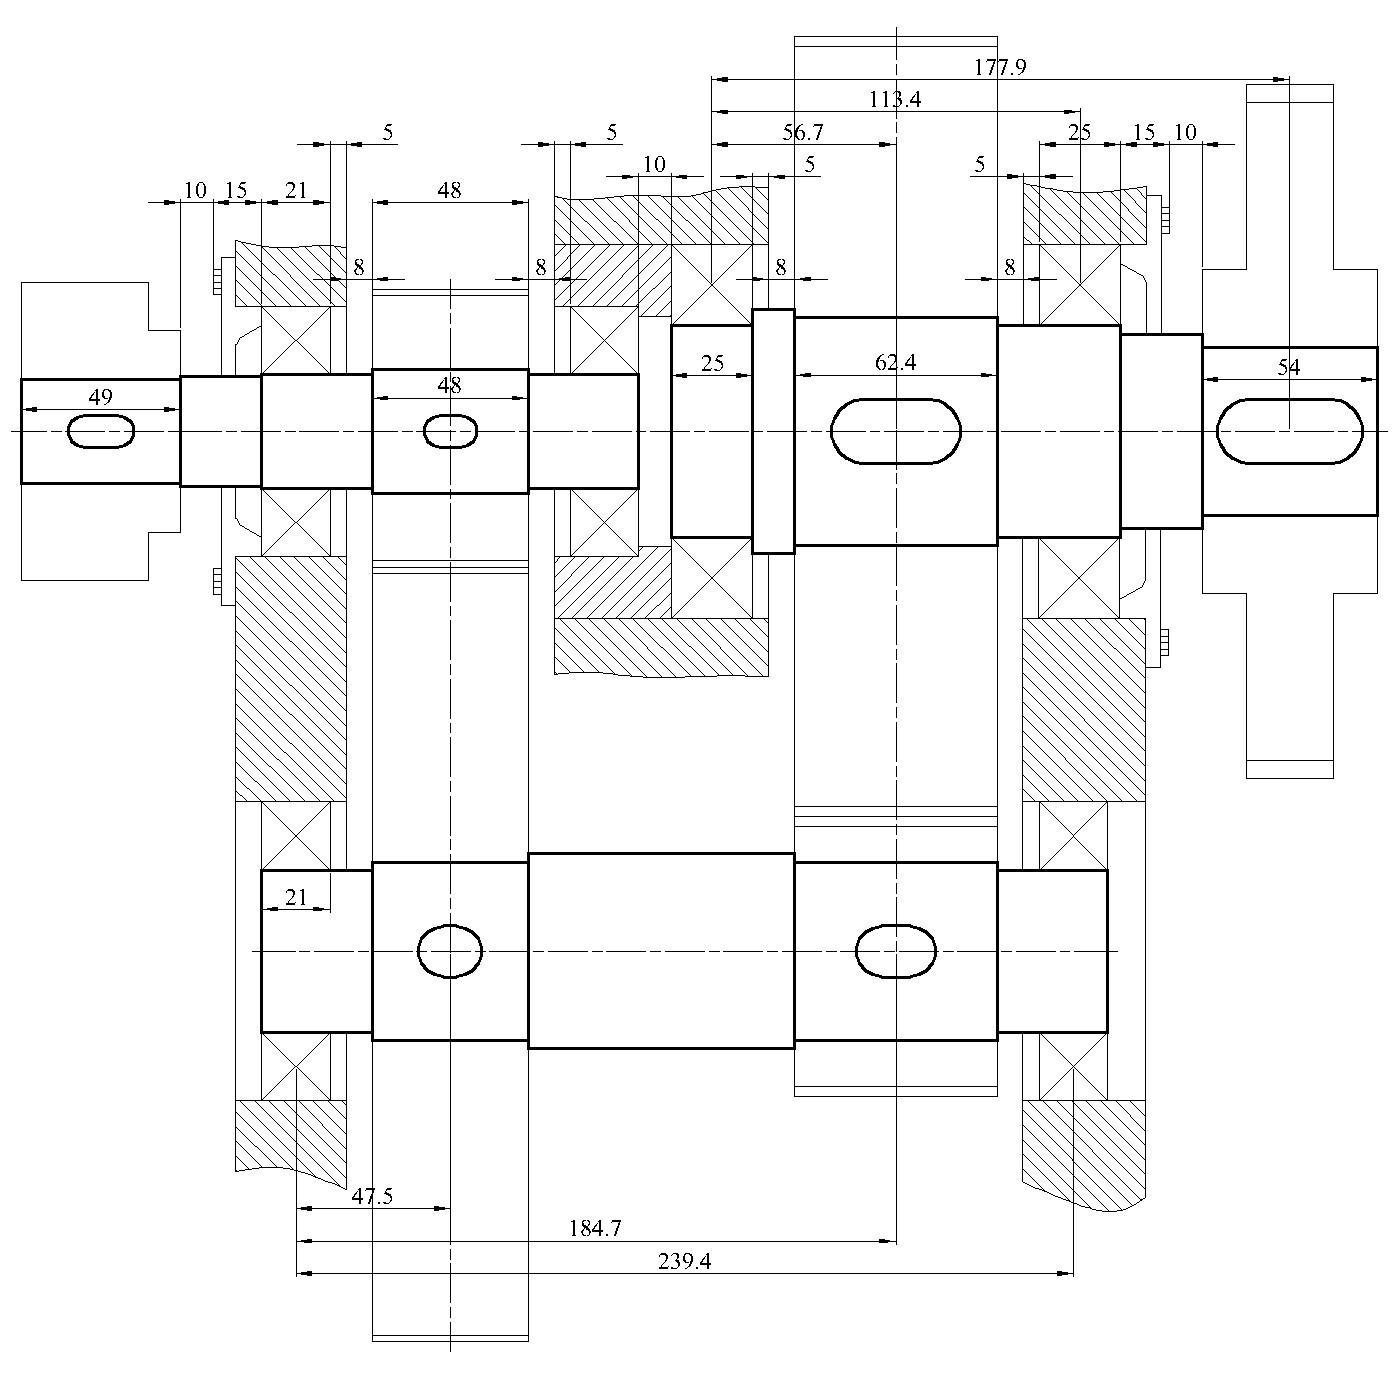
\includegraphics[width=\linewidth]{gearbox structure}
%	\caption{Structure of the speed reducer}
%	\label{gearbox}
%\end{figure}
%
%\section{Structure design for stress concentration factor and increasing life span}

